\documentclass[11pt,a4paper,openright,twoside]{report}

\usepackage[pdftex]{graphicx}
\usepackage[english]{babel}
\usepackage[T1]{fontenc}
\usepackage[utf8]{inputenc}
\usepackage{url}
\usepackage[hidelinks]{hyperref}
\usepackage{setspace}

\usepackage{fancyhdr}
\usepackage{indentfirst}
\usepackage{newlfont}
\usepackage{xcolor}

\definecolor{mygreen}{rgb}{0,0.6,0}
\definecolor{mygray}{rgb}{0.5,0.5,0.5}
\definecolor{mymauve}{rgb}{0.58,0,0.82}
\definecolor{pred}{rgb}{0.9,0,0}
\definecolor{light-gray}{gray}{0.95}
\usepackage{listings}
\lstset{ 
	backgroundcolor=\color{light-gray},   % choose the background color; you must add \usepackage{color} or \usepackage{xcolor}; should come as last argument
	breakatwhitespace=false,         % sets if automatic breaks should only happen at whitespace
	breaklines=true,                 % sets automatic line breaking
	escapeinside={\%*}{*)},          % if you want to add LaTeX within your code
	extendedchars=true,              % lets you use non-ASCII characters; for 8-bits encodings only, does not work with UTF-8
	keepspaces=true,                 % keeps spaces in text, useful for keeping indentation of code (possibly needs columns=flexible)
	basicstyle=\footnotesize,        % the size of the fonts that are used for the code
	numbers=left,                    % where to put the line-numbers; possible values are (none, left, right)
	numbersep=5pt,                   % how far the line-numbers are from the code
	%language=XML,                	 % the language of the code
	commentstyle=\color{mygreen},    % comment style
	keywordstyle=\color{blue},       % keyword style
	numberstyle=\tiny\color{mygray}, % the style that is used for the line-numbers
	stringstyle=\color{pred},
	rulecolor=\color{black},         % if not set, the frame-color may be changed on line-breaks within not-black text (e.g. comments (green here))
	stringstyle=\color{mymauve},     % string literal style
	tabsize=4		%modify tab space, default too wide
}


\usepackage{amssymb}
\usepackage{amsmath}
\usepackage{latexsym}
\usepackage{amsthm}

\oddsidemargin=30pt \evensidemargin=20pt%impostano i margini
\usepackage[htt]{hyphenat} %per andare a capo nei typescript
\hyphenation{uni-ver-sity
	uni-ver-sit-ies
	how-ever
	ma-nu-script
	ma-nu-scripts
	re-ci-pro-city
	through-out
	some-thing
	al-tern-ate}%serve per la sillabazione: tra parentesi 

\pagestyle{fancy}\addtolength{\headwidth}{20pt}
\renewcommand{\chaptermark}[1]{\markboth{\thechapter.\ #1}{}}
\renewcommand{\sectionmark}[1]{\markright{\thesection \ #1}{}}
\rhead[\fancyplain{}{\bfseries\leftmark}]{\fancyplain{}{\bfseries\thepage}}
\cfoot{}

%\linespread{1.3}                     

\begin{document}
	
	\thispagestyle{empty}
\begin{titlepage}

\vspace*{-1.5cm}
\begin{center}
  \large
  \textbf{ALMA MATER STUDIORUM - UNIVERSIT\`A DI BOLOGNA}\\
  
  \hrulefill\\
  
  \textbf{SCHOOL OF ENGINEERING AND ARCHITECTURE}\\
  \vspace*{.75cm}
  
  
  Department of Computer Science and Engineering - DISI\\
  Laurea Magistrale (Second Cycle Degree) in Computer Engineering\\
  
  \vspace*{1.2cm}
  
  
  \textbf{PROJECT WORK}\\
  \vspace*{.4cm}
  for\\
  \vspace*{.4cm}
  INFORMATION SECURITY M\\

  \vspace*{2cm} \LARGE
  \textbf{titolo titolo titolo titolo titolo}\\
 \end{center}
 
 \vspace*{3cm}
 
 \begin{flushleft}
  \textbf{CANDIDATE}\\ Giada Martina Stivala \\
\end{flushleft}

\vspace*{-2cm}

 \begin{flushright}
  \textbf{SUPERVISOR}\\ Chiar.ma Prof.ssa Rebecca Montanari \\
 \end{flushright}


\vspace*{2cm}

\begin{center}
	\textbf{
  Academic Year 2017/2018\\
  }
\end{center} 
\clearpage
\end{titlepage} 
	\clearpage{\pagestyle{empty}\cleardoublepage}%non numera l'ultima pagina sinistra
	
	\pagenumbering{roman}                   %serve per mettere i numeri romani
	\chapter*{Abstract}

\noindent This Project Work on Information Security focuses on regulating personal data disclosure among third parties, providing a simple implementation within the Android framework. To increase their privacy, data owners can purposefully create \textit{Sticky Policies}, metadata to describe which users or services can access the personal information they stick to.

First, we describe the state of the art in terms of literature and existing algorithms for \textit{Sticky Policy} implementation; then, we analyze the available concrete solutions and their weaknesses. Finally, we present our solution and its features, including considerations about future improvements.

In the last chapter, we show performance measurements and comparisons to support our work and decisions.
	\addcontentsline{toc}{chapter}{Abstract}
	\clearpage{\pagestyle{empty}\cleardoublepage}

	\tableofcontents                        
	\clearpage{\pagestyle{empty}\cleardoublepage}
	\pagenumbering{arabic}                  %mette i numeri arabi

	\chapter{Introduction}
\label{Intro}
\thispagestyle{empty}

\noindent 
Personal data increasingly fuel Internet applications development and spread, especially since the birth and diffusion of Big Data. Users are often unaware of the gathering, processing and storage of their data, mostly because of the obfuscation behind license agreements and the technical notions necessary to understand these processes. Data may also be moved across country borders, to be processed under different laws and regulations, with processing systems so complex to ultimately make it impossible to understand which service provider had the right to process what.

Leaving out the risks originating for accidental data disclosure by such applications, for example due to security breaches, users may wish to increase their data protection, especially in fields as medical care and financial services. More specifically, we would like a tool to selectively reduce data disclosure, preventing unwanted usage from third parties.

Current solutions include state laws about data usage and protection, business frameworks and service-level agreements, which prove to be inefficient and ineffective. Many research studies have thus advanced the suggestion of a different tool, called \textit{Sticky Policies}, to ensure data protection and control their disclosure. \textit{Sticky Policies} are essentially machine-readable metadata which specify the correct usage of the data they travel with \cite{pearson2011sticky}: through encryption, they prevent policy non-compliant use.

In this project work, I start by analysing the most recent and relevant proposals about this matter, comparing different technical approaches and existing solutions. Then, I introduce a solution of my own, which tackles this issue within a limited scope of action. Finally, I present my conclusions about this work.


\iffalse
- internet funziona sempre più producendo risultati a partire da dati personali, e questa tendenza sta aumentando grazie al diffondersi di big data
- gli utenti sono, nella maggior parte dei casi, ignari dell'uso che viene fatto dei loro dati personali, e in ogni caso, spesso, tali servizi avvengono sotto legislazioni diverse, o avvengono per conto di ulteriori terze parti che potrebbero non rispettare i permessi inizialmente accordati.
- questi costituiscono dei rischi per la violazione della privacy e in generale potrebbero costituire una vulnerabilità, esposizione, degli utenti agli attacchi su internet.
- vorremmo che fosse possibile per gli utenti scegliere selettivamente cosa condividere, dando loro la possibilità di limitare la diffusione dei loro dati personali dovuta a servizi esterni.
- per fare ciò si propone l'uso di sticky policies, ossia metadati che restano agganciati ai dati a cui si riferiscono e danno indicazioni sul loro corretto utilizzo.
\fi
	\chapter{cap 2}
\label{capitolo2}
\thispagestyle{empty}

\section{sezione} Lorem ipsum dolor sit amet, consectetur adipiscing elit, sed do eiusmod tempor incididunt ut labore et dolore magna aliqua. Ut enim ad minim veniam, quis nostrud exercitation ullamco laboris nisi ut aliquip ex ea commodo consequat. Duis aute irure dolor in reprehenderit in voluptate velit esse cillum dolore eu fugiat nulla pariatur. Excepteur sint occaecat cupidatat non proident, sunt in culpa qui officia deserunt mollit anim id est laborum.Lorem ipsum dolor sit amet, consectetur adipiscing elit, sed do eiusmod tempor incididunt ut labore et dolore magna aliqua. Ut enim ad minim veniam, quis nostrud exercitation ullamco laboris nisi ut aliquip ex ea commodo consequat. Duis aute irure dolor in reprehenderit in voluptate velit esse cillum dolore eu fugiat nulla pariatur. Excepteur sint occaecat cupidatat non proident, sunt in culpa qui officia deserunt mollit anim id est laborum.
	\chapter{A simple implementation}
\label{chapter3}
\thispagestyle{empty}

\noindent First, we set up the necessary entities to implement \textit{Sticky Policies}: an Android client and a web server. The client was developed using Android Studio and emulated through the Android Emulator with a Nexus 5X device running Android 7.0 and API level 24. The Trusted Authority was developed using Eclipse and run on Apache Tomcat 8; the communication was implemented through HTTP protocol.

The app was also tested in a Samsung tablet (SM-T230) running Android 4.4.2 and API level 19, to test performance on a real device with lower level API and operating system, together with a different screen dimension.

In this solution, \textit{Sticky Policies} are realized via XML files and paired with personal data through the combination of symmetric and asymmetric cryptography. This approach is presented in \cite{pearson2011sticky}, and an example XML policy was created taking as a reference the one presented in the same paper. Following this specification, we present a protocol for the communication of two Android clients, called for simplicity Alice and Bob. 

Alice generates an XML policy to regulate data access, encrypting it with a symmetric key generated locally. The policy and the key are then encrypted with the Trusted Authority's public key and signed by Alice. Purposely, Alice should obtain the public key of the Trusted Authority and also a key pair for herself: in our solution, we use self-signed X509 Certificates generated by combining the Java Cryptography Architecture and the Bouncy Castle cryptography APIs for Java. Alice thus contacts the Trusted Authority to obtain its public key, and shares her own if the Trusted Authority is not the issuer of her certificate.

Bob obtained Alice's encrypted data and an attached policy in clear text, together with other encrypted data to guarantee integrity, confidentiality and non-refusal of the policy and data. In particular,
\begin{itemize}
	\item Integrity is granted for the policy in plain text by sharing its digest, encrypted with the Trusted Authority's public key.
	\item Confidentiality is granted both for the personal data, which is shared encrypted, and for its symmetric key which is encrypted together with the policy's digest
	\item Non-refusal is granted for all of the shared data thanks to the signing function applied by the data owner.
\end{itemize}

To decrypt Alice's data, Bob must follow these steps:
\begin{itemize}
	\item Bob asks the Trust Authority to release the symmetric key, presenting the encrypted data signed by Alice.
	\item The Trust Authority evaluates the policy and Bob's reliability, submitting some challenges for him to complete.
	\item If trusted, Bob receives the symmetric key to decrypt Alice's personal data.
\end{itemize}

Data is exchanged through POST requests over a channel which is assumed to be secure.

Once the Trust Authority receives a request from the client, it checks the correct specification of the policy before proceeding to decrypt and verify the payload received. This operation is performed by a server-side parser which matches the XML file with a standard XSD grammar. In case of errors, no symmetric key is released.

The specification of the XSD grammar can be found in Appendix \ref{appendixA}. 

\section{Program flow and architecture}
We start by analysing the application flow before data is shared, given that Alice has installed an instance of the StickyPolicyApp.

The data owner can either share a simple text message (shown in Figure \ref{fig:share-text}) or a regular file inside his phone (for example an image, in Figure \ref{fig:share-img}), chosen through a picker. Consequently, the underlying application generates a fitting policy depending on the data shared and on the owner itself, which is then passed to the next \texttt{Activity} for encryption and sharing. In this solution, for the sake of simplicity, the generated policy contains mock data, except for the X509 Certificate serial number and the data type. Possible future works include adding an interactive policy generator to allow the user to define sharing constraints.
\begin{figure}
	\centering
	\begin{minipage}{0.35\textwidth}
		\centering
		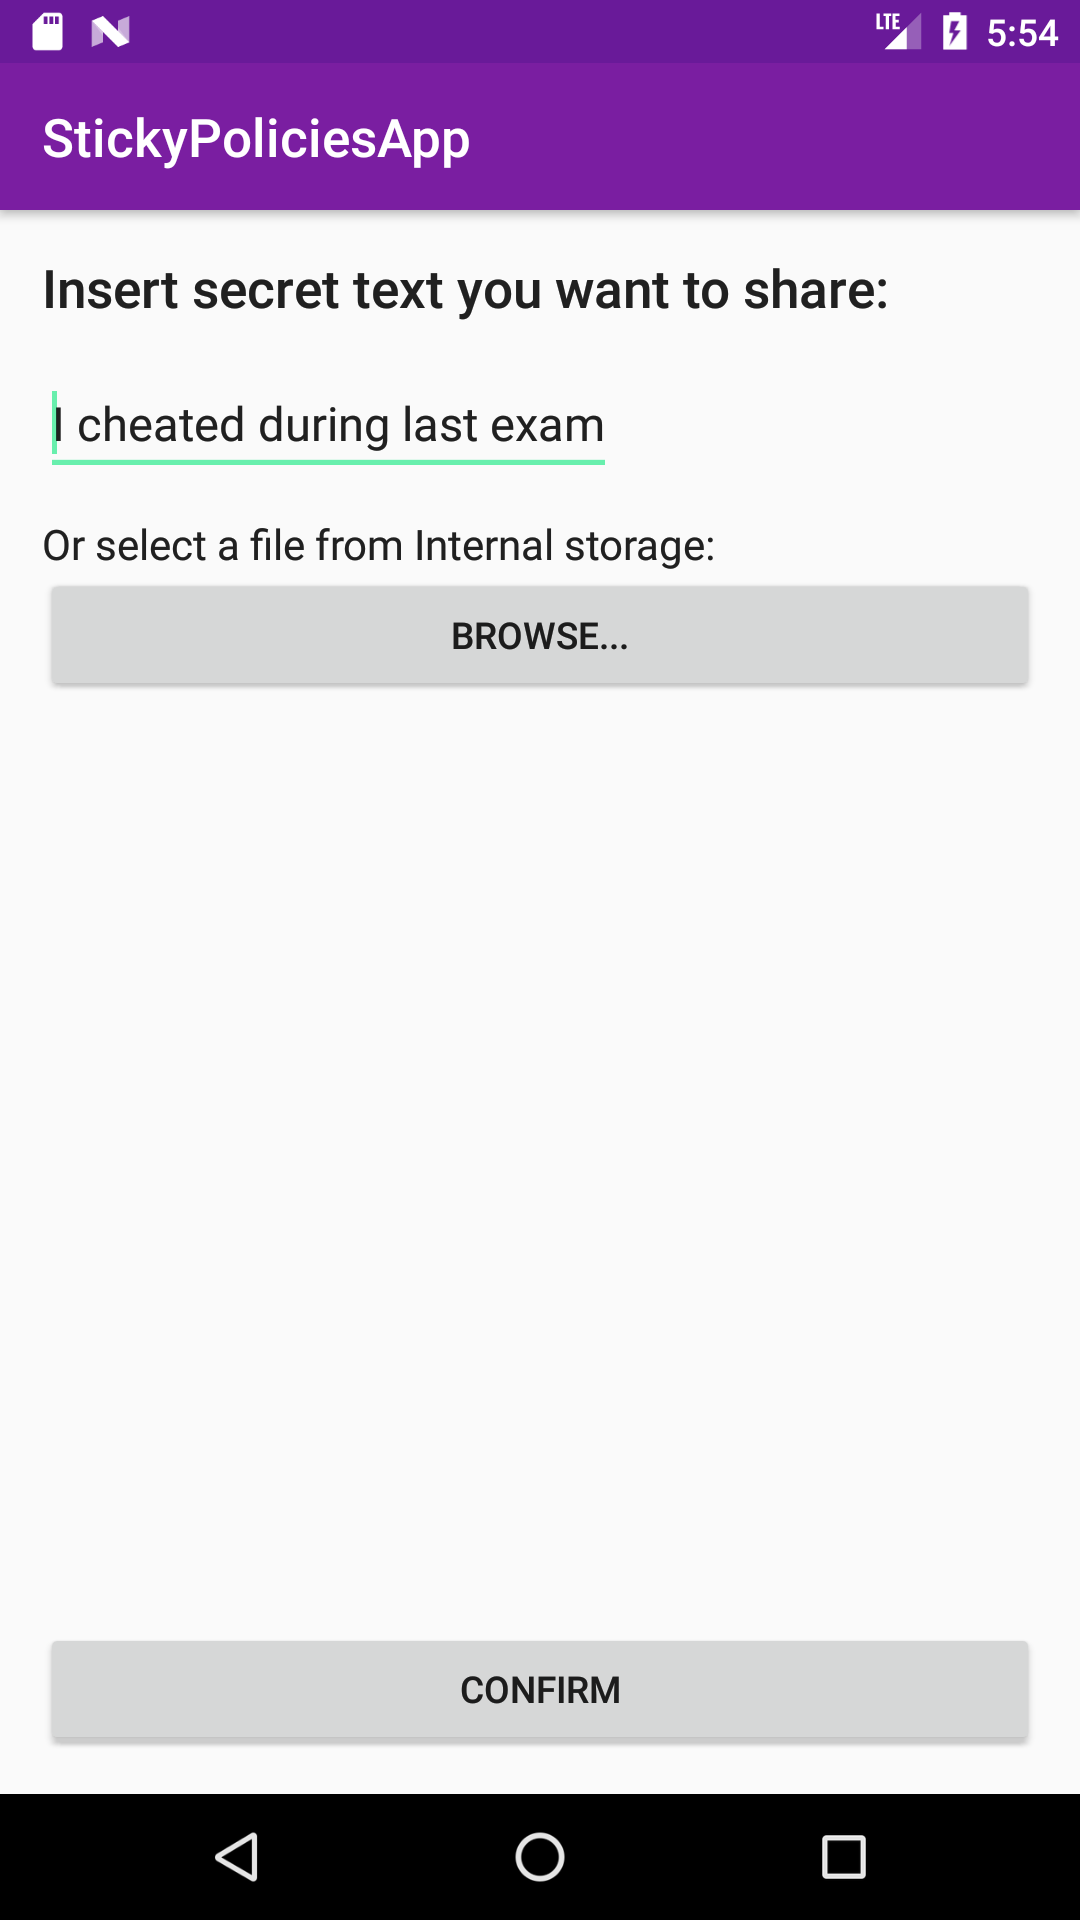
\includegraphics[width=0.9\textwidth]{ShareData-text.png} % first figure itself
		\caption{Sharing secret text}
		\label{fig:share-text}
	\end{minipage}
	\begin{minipage}{0.35\textwidth}
		\centering
		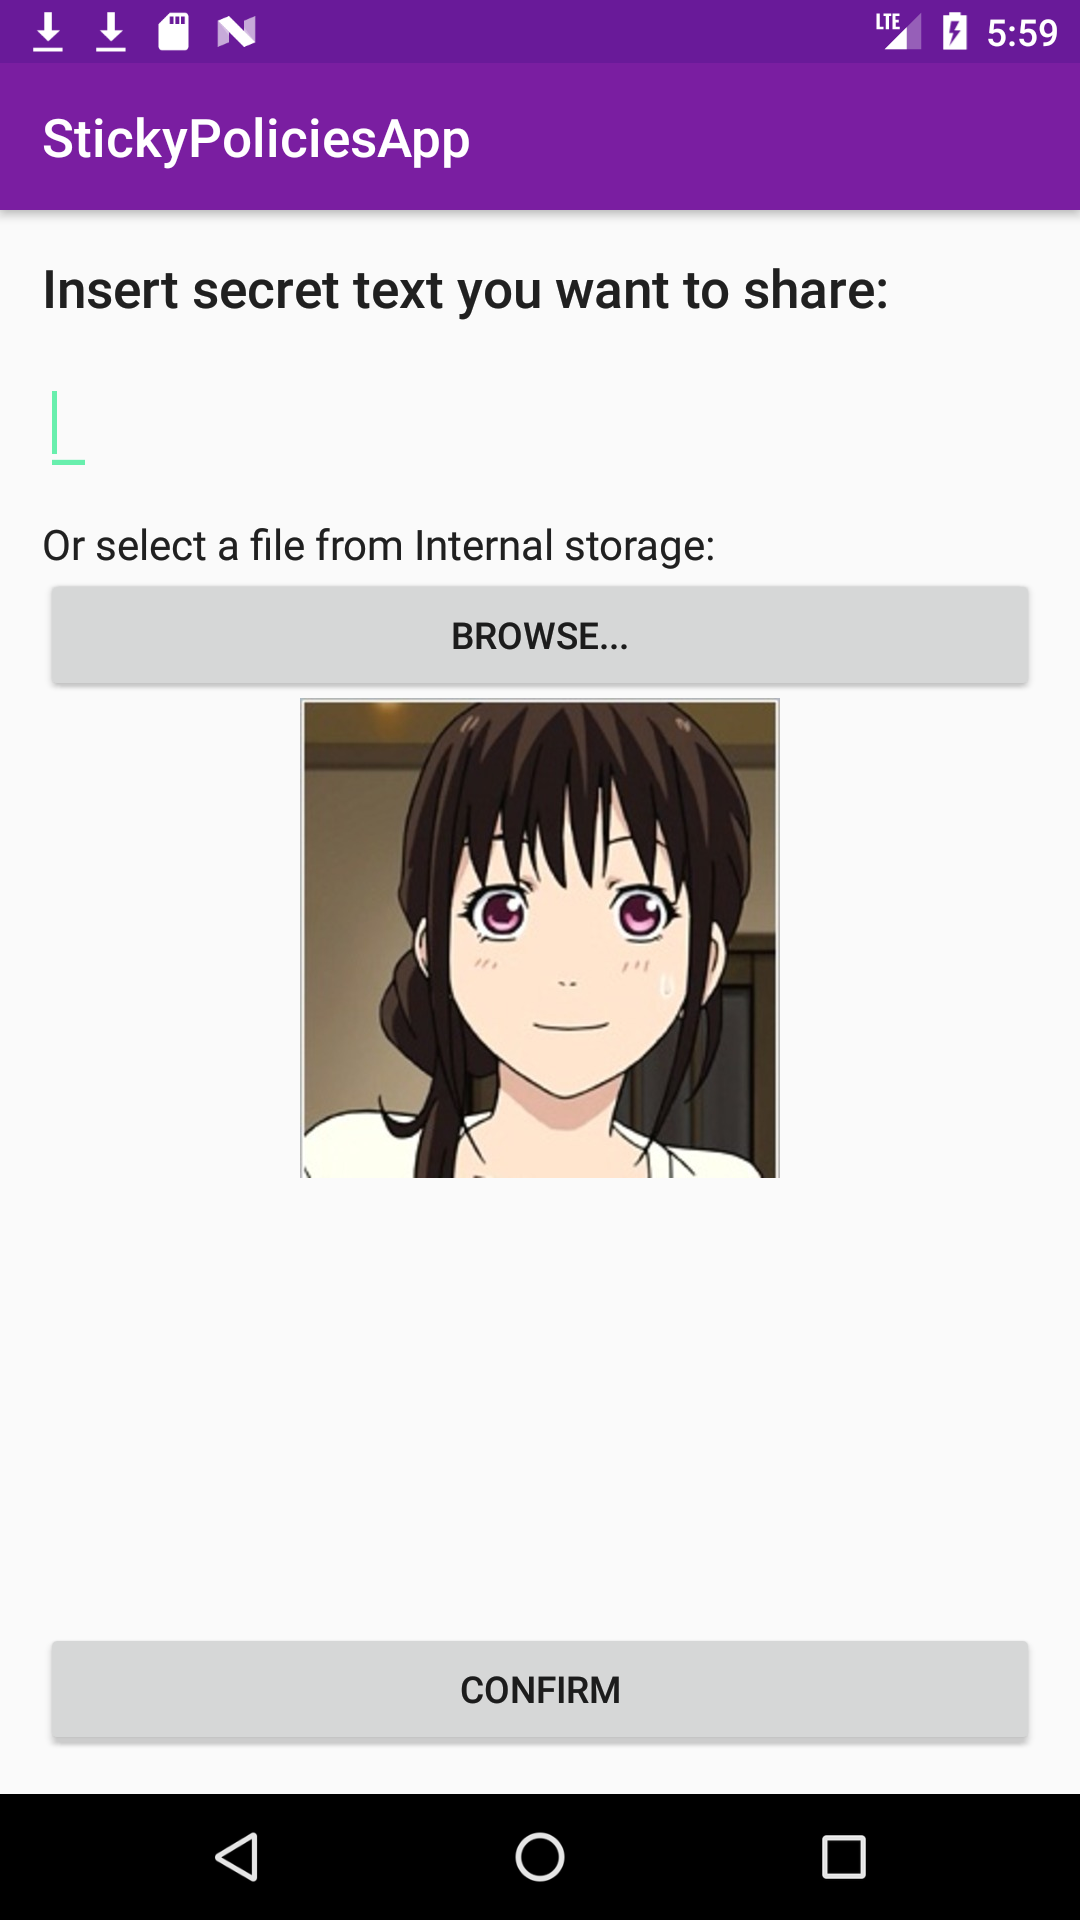
\includegraphics[width=0.9\textwidth]{ShareData-image.png} % second figure itself
		\caption{Sharing a personal image}
		\label{fig:share-img}
	\end{minipage}
\end{figure}

A certificate exchange is then initiated between the client and the server, to perform both signature and encryption inside the app and to allow the Trusted Authority to run security checks on data, when requested access by third parties. Subsequently, the policy and data are processed following the specification presented in \cite{pearson2011sticky}: the data is encrypted with a one-time-use symmetric key generated at the moment, and together with a digest of the policy they are first encrypted with the public key of the Trusted Authority, then signed with the data owner's private key.

It is now possible for Alice to safely share her data, sending it to Bob. Data is transferred inside the body of POST requests in JSON form. To safely and efficiently perform data serialization and deserialization we used the \texttt{com.google.code.gson} library and implemented an ad-hoc private class to hold both policy and encrypted data in a single GSON object. For this purpose, we tested also the libraries \texttt{org.json} and \texttt{org.jabsorb}, which though proved to be unsuitable and less efficient.

Let's now consider the StickyPoliciesApp to be running on Bob's device, and to have just received a secret message from Alice. Bob forwards to the Trusted Authority the plain-text policy together with the signed key and digest, removing the encrypted personal data from the new request body. At this point, the Trusted Authority may check Bob's reliability and submit a few challenges to prove it, eventually disclosing the symmetric key to access Alice's secret message.

Both the communication and the cryptographic primitives are performed inside \texttt{AsyncTask}s: this keeps the main UI thread responsive and prevents the app from freezing due to intensive, network-dependent computation.

\subsection{Android Client Implementation}
The StickyPoliciesApp consists of a few \texttt{Activities}. The launcher allows either to send private data or to access received messages, but can be extended to include new functionalities, as the aforementioned policy editing.

Navigation within the activities is made through explicit \texttt{Intent}s: as specified within the Android security guidelines, implicit \texttt{Intent}s may introduce security hazards as it is not known which service will respond to the intent, and the user has no control over it.

The first activity is in charge of data sharing: once the data type of the shared information is determined, it requests from the \texttt{CryptoUtils} class the data owner's certificate to retrieve its serial number, edits the sticky policy so that it matches both personal data type and certificate SN; finally, it creates a \texttt{Bundle} to pass these objects to the following activity, invoked explicitly.

The \texttt{PolicyClient} class is in charge of communication operations: it performs a certificate exchange with the Trusted Authority and it encrypts data, sending them to Bob. These operations are performed via dedicated \texttt{AsyncTask}s which are started in the \texttt{onResume()} method, so that the main UI thread is built without delay. Both tasks simply prepare data for the HTTP request, invoke a library function to handle it at a lower level and parse the results. For example, this is how the data owner's certificate is shared:
\lstinputlisting[caption={AsyncTask from PolicyClient class},label={list:SendCert},language=java]{SendEncrData-excerpt.java}

\noindent where \texttt{NetworkUtils} is a public class exposing \texttt{static} methods for network management. As for data encryption, operations are performed following the specification in \cite{pearson2011sticky}, and an excerpt of the code is shown in Listing \ref{list:EncryptData}.
\lstinputlisting[caption={Excerpt from PolicyClient class},label={list:EncryptData},language=java]{SendEncrData-excerpt2.java}

In Listing \ref{list:EncryptData}, we omit try-catch blocks for error handling. To stop the application flow when fatal errors occur (e.g. data encryption fails), a high-level \texttt{SecurityException} is thrown and a message is delivered to the user, prompting him to retry later. The same approach is applied inside the whole application: errors are managed locally and a high-level message is shown to the user in case of critical exceptions.

Finally, Bob can access the received data in a third \texttt{Activity}, in which he shares part of his \texttt{EncryptedData} with the Trusted Authority and receives back the encrypted symmetric key and the initialization vector.

\subsection{Java Server Implementation}
We realized the Trusted Authority as a web server exposing two services, reachable via the corresponding servlets hosted in the servlet container Apache Tomcat: \texttt{PolicyServer/certificates} and \texttt{PolicyServer/access}.

The first servlet is in charge of sharing the Trusted Authority's \texttt{X509 Certificate} in \texttt{PEM} format, and it also manages the data owners who register to the TA. Certificates are accepted in \texttt{PEM} format. The state is kept server-side inside the \texttt{ServletContext}, which is bound to the container's life cycle rather than to the single user or session, and certificates are stored in a \texttt{HashMap<BigInteger, X509Certificate>}. The \texttt{HashMap} is a data structure which allows quick access and prevents duplicate addition: thus, when a user "Bob" asking for data access sends a message in which the certificate SN does not match any of the \texttt{HashMap} entries, the request will be refused. This behaviour requires the state to be shared between the two servlets, possible thanks to the use of a Java Bean.

The second service provides data access: JSON data is received in POST requests, containing plain-text policies together with signed key and digest. The servlet checks validity and integrity of the policy, verifying the signature and decrypting the obtained data to retrieve the symmetric key. If any of these procedures fails, the entire process is interrupted and the access request is refused with an error code corresponding to the cause of the error. For example,
\lstinputlisting[caption={Excerpt from DataAccessServlet class},label={list:DataAccess-error},language=java]{DataAccessServlet-excerpt.java}

In a future improved version of this app, the symmetric key could be encrypted with Bob's public key before sharing, requiring Bob to register at the Trusted Authority first. This development depends on the dimension of encrypted symmetric key together with the initialization vector, which is currently shared every time together with the key; their overall size must not exceed the size of the modulus for the generated Trusted Authority's key pair. Other possible improvements include the implementation of policy-specified \texttt{action}s, as for example informing the data owner when data access is granted.

As it is, our web server shows the same weaknesses we described in the previous chapter, regarding secure storage and network attacks; moreover, additional weaknesses are introduced by the communication with a potential malicious client. In other words, no check is performed on the payload (content-type, dimension, user-agent) and the client is considered to be always trusted.

\section{Structure of an XML policy}
The policy file is constructed by the data owner in order to specify which set of users can access her data. Policies are shared over the internet as strings, thus formats like XML or JSON represent the best choice in terms of interoperability and ease of use. Choosing the XML format over a new, custom implementation for Sticky Policies enables the use of well-known corroborated libraries and best practices, available due to XML widespread. Moreover, the document format is designed for data transfer and to be self-descriptive: its structure and content can easily be regulated through grammars and specifications.

Sticky Policies have been designed with a general and comprehensive structure, so as to allow broader usage than the one proposed in this solution. The main components of a Sticky Policy are the following:
\begin{itemize}
	\item List of the Trusted Authorities where Bob can ask for data access. They are specified by Alice and they include all the servers in which she registered her certificate.
	\item Details about the Data Owner, which are used server-side to retrieve the correct certificate and public key.
	\item One or more policies, specifying fine-grained constraints about the attached data. They may vary in target, time validity, requirements, etc, specifying different requirements for different target users or services. The complete specification is available in Appendix \ref{appendixA}.
\end{itemize}

Each field within the policy is detailed in the grammar, where are specified constraints about its values, position, number or occurrences, etc. Some of these constraints describe logical evidence - e.g. each policy refers to a single Data Owner:
\lstinputlisting[label={list:XSDgrammar-ownerExcerpt},language=XML]{PKIstickypolicy-excerpt.xsd}
as well as real-world constraints - e.g. days can range from 1 to 31:
\lstinputlisting[label={list:XSDgrammar-dateExcerpt},language=XML]{PKIstickypolicy-excerpt1.xsd}
and finally programming constraints - e.g. a \texttt{X509Certificate}'s serial number is represented throgh a \texttt{BigInteger}, which is mapped to a \texttt{xs:unsigned Long}:
\lstinputlisting[label={list:XSDgrammar-snExcerpt},language=XML]{PKIstickypolicy-excerpt2.xsd}

\subsection{XML Validation and Parsing}
Policies are parsed server side: this control step includes validation, i.e. checking both syntax and semantics of the document. In Java, it is possible to realize an XML parser through a \texttt{SAXParser}, a low-level implementation which scans the whole document and for each start tag and end tag found fires and event, handled by callback methods to retrieve the content between the tags. While this allows to gain in efficiency and is suited also to parse large documents, it constitutes and ad-hoc tailored solution, unsuited for dynamic environments.

Document parsing is performed by a \texttt{ContentHandler}, in which callback methods are defined: we chose to implement them via the subclass \texttt{DefaultHandler} and its methods \texttt{startElement}, \texttt{characters}, \texttt{endElement}.

In our solution, we implemented also a \texttt{XMLErrorChecker} for error handling. This parser provides three different types of errors: fatal errors, errors and warnings, although by default only fatal errors are fired. In these cases, the parser cannot continue and the method performs \texttt{System.exit(1)}, while nonfatal errors are generated when the document fails some validity constraints (e.g. invalid tag, tag not allowed...). We redefined the default behaviour by firing \texttt{SAXException}s also for nonfatal errors, due to the considerable importance of having a well-formed and valid document. These exceptions are then caught by the caller, at a higher level of the call stack, and handled by refusing the data disclosure request.

\section{About cryptography}
Cryptography constitutes a considerable part of the whole project. All cryptographic functions are realized as static, and are accessible as if they were an external library both in the client and server. Both of them rely on the Java Cryptography Architecture together with Bouncy Castle APIs. They include X509 Certificate generation, sign, verify and asymmetric encryption operations as well as symmetric key generation and encryption. Finally, it is possible to generate also message digests. Provider names, algorithms and key size are fixed parameters within the application and it is not possible for the user to choose any; future developments may give her the chance to choose between algorithm implementations corresponding to different levels of security.

\subsection{Message Digests}
Computing message digests is an important part of this security protocol: first, it proves policy's integrity by matching the received digest with the one computed server-side from the plain-text policy; second, it lowers the size of the data to be encrypted, giving it a fixed dimension of 32 bytes. In fact, policy files can potentially grow in size and, were the policy not to be hashed before asymmetric encryption, it could introduce a weakness within RSA's encryption method. If the overall dimension of the symmetric key and policy were greater than the dimension of the modulus for asymmetric encryption, either the dimension of the modulus would increase, or encryption would be performed after splitting the whole data into blocks of size lower than 1024 bits.

The cryptographic hash function used in this project is the SHA-256 function, and the implementation is the one provided by the class \texttt{java.security. MessageDigest}. To obtain a message digest it is necessary to follow a three-step procedure: first, an instance of \texttt{MessageDigest} is retrieved for the specified algorithm; then, it receives as input the text to hash and, finally, the \texttt{digest()} function is called.

\lstinputlisting[caption={Excerpt from CryptoUtilities class},label={list:MessageDigest},language=java]{MessageDigest.java}

Digests are compared with the \texttt{MessageDigest.isEqual(byte[] first, byte[] second)} function, which does a simple byte compare, as reported by the Java documentation.

Switching from SHA-256 to SHA-512 could increase efficiency in our case, thanks to the chosen device having a x86\_64 architecture and being SHA-512 based on 64-bits words.  Furthermore, this would not pose any problem in terms of API availability since both of them are available since API level 1+. Switching to SHA-512 would double the size of the produced digest, leaving only 64 bytes of space to encode the symmetric key. Keeping into consideration previous observations about having a maximum data size of 128 bytes, we have preferred a smaller message digest also in terms of bandwith consumption and foreseeing a possible symmetric-key dimension increase. Initialization vectors may also be shared in the remaining 64 bytes, and their dimension may vary depending on the encryption algorithm.

\subsection{X509Certificates}
\label{subsec:x509cert}
The Bouncy Castle library provides functionalities to create self-signed X509 Certificates, chosen for the sake of simplicity. In a more realistic implementation, certificates should be issued by a Certification Authority, and the Trust Authority should additionally perform certificate verification (e.g. expiration and revocation). To construct the \texttt{X509Certificate}, we use 1024-bit asymmetric keys generated for the RSA algorithm, and the Bouncy Castle security provider. 2048-bit long keys could be more appropriate depending on the confidentiality of the information shared, on the mobile device and network possibilities.

Both the Trust Authority and the Data Owner need a certificate to store and share securely their public key. \texttt{X509Certificate} construction follows a similar procedure for the both of them, with few exceptions. In case the Trusted Authority works also as a Certification Authority, then 

\lstinline[language=java]!BasicConstraints constraints = new BasicConstraints(true);!

\noindent while for the mobile device we use a \texttt{false} parameter. Moreover, in both cases, certificates are created and handled as singleton objects, to prevent inappropriate duplicates: the methods and fields to generate and store certificates are \texttt{private}, and their content can be retrieved through accessor methods, which also control the instance creation.

Among the Bouncy Castle library there is the LightCrypto implementation \cite{LightCrypto}, available for phones or devices with limited computational power. It allows the creation of key pairs and certificates, but their interoperability with the Java Cryptography Architecture is limited and so a conventional certificate implementation is preferred. 

Certificates are shared from both client and server in PEM format using a \texttt{JcaPEMWriter} for serialization and a \texttt{CertificateFactory} for deserialization. This format has been preferred to ASN.1 as easier to send in a HTML request body, it being a \texttt{String} rather than a \texttt{byte[]}.

\subsection{Asymmetric Key Generation and Encryption}
As mentioned in subsection \ref{subsec:x509cert}, asymmetric keys are generated with a modulus length of 1024 bits. We use a \texttt{KeyPairGenerator} specifying both the algorithm (AES) and the security provider (Bouncy Castle).

\lstinputlisting[caption={Excerpt from CryptoUtilities class},label={list:KeyGen},language=java]{KeyGenExcerpt.java}

In this project, asymmetric encryption and signature is used to communicate with the Trusted Authority, and as such the same cryptographic methods are implemented server side. Security considerations in this matter have their basis in the RSA Cryptography Specification \cite{rfc8017}.

The security protocol described in \cite{pearson2011sticky} requires to implement the signature with appendix scheme since it appends a message and its signature when communicating to the Trusted Authority. For the sign and verify methods we chose the \texttt{SHA256WithRSA} algorithm. 

Regarding asymmetric encryption, which is performed before the sign operation, the \texttt{RSA/ECB/OAEPPadding} algorithm was preferred to the \texttt{RSA/ECB/PKCS1Padding} due to proven resistance to chosen-ciphertext attacks. The reason is related with the predictability of padding schemes applied during encryption, and in particular when the plain text dimension is higher than the dimension of the modulus. In these cases, the original text is split in many blocks, which are then hashed and padded before encryption to avoid a potential attacker to recombine them and still verify successfully.

In the previous and following subsections has been highlighted how it was better to have an overall data size lower than the modulus: in fact, it is good practice not to rely on asymmetric encryption for large data also for its inefficiency, but proper choice of the implementation algorithm guarantees that no additional weakness is introduced in case it should happen.

\subsection{Symmetric Key Generation and Encryption}
In this subsection, we will refer always to cryptographic operations happening on the Android devices, since the Trusted Authority never receives personal data.

The specification in paper \cite{pearson2011sticky} asks for a symmetric one-time-use key to encode personal data. Symmetric keys can be generated via a \texttt{KeyGenerator} with an algorithm-specific initialization, not providing \texttt{SecureRandom} to rely on the implementation of the highest-priority installed provider. This raises the reliability of the proposed solution, as symmetric keys are never reused and are unrelated. The available algorithms for encryption and key generation depend on the chosen security \texttt{Provider}, which is in our case the Bouncy Castle provider. Available key generation algorithms include AES for symmetric encryption, in particular AES/ECB and AES/GCM/NOPADDING: since the former has known weaknesses and it is not suited to large-size file encryption, we considered switching to another \texttt{Provider}, namely AndroidOpenSSL provider. A working example using AES/ECB is shown in Listing \ref{list:ECBencryption}. Invocation must specify \texttt{Cipher.ENCRYPT\_MODE} or \texttt{Cipher.DECRYPT \_MODE} to perform either encryption or decryption.

\lstinputlisting[caption={Example code with AES/ECB processing on Android device},label={list:ECBencryption},language=java]{EncryptSymmetricECB.java}

The Bouncy Castle provider also offers implementations for several Password Based Encryption methods, using AES/CBC with different key lengths, salt and padding options. We did not consider any of those algorithms as they are out of the scope of this project: encryption must be performed with a one-time-use secret, while using a fixed password would definitely reduce the security level. Moreover, PBE requires many iterations in order to process a secure derived key (around 100 000 or 200 000), which could impact on efficiency and performance.

The implemented solution makes use of a AES/CBC/PKCS5Padding  algorithm is available with the AndroidOpenSSL provider: the Cipher Block Chaining operation mode is more secure than Electronic Codebook, and is suited to work in this context as a block cipher mode. Padding is needed due to unpredictable size of the policy, which may not be a multiple of the block size (128 bits). In the Cipher Block Chaining mode an initialization vector is needed at the beginning of each encryption / decryption process to be XOR'd with the first block of plain text: to obtain it we rely on the Java class \texttt{SecureRandom}, and we create a initialization vector of the same size of a block in CBC. It is worth highlighting how we ask \texttt{secureRandom.nextBytes(iv);} to generate the initialization vector to avoid reuse of previous configurations; weaknesses  may also be introduced from a repetitive initialization value for the \texttt{SecureRandom} present in some implementations. Furthermore, when creating a symmetric key we need to specify \texttt{"AES"} as input parameter, while for the encryption and decryption methods we add the initialization vector:

\lstinputlisting[caption={Example code with AES/CBC processing on Android device},label={list:CBCencryption},language=java]{EncryptSymmetricCBC.java}

The initialization vector must be shared between Alice and Bob to allow correct decryption. Despite it not being a secret, initialization vector reuse or publication may introduce weaknesses in the cipher mode, leaking information about the first plain text block. On the other side, initialization vector reuse or publication may be desirable in terms of network and bandwith consumption: thus, it is suggested that each solution is tailored to the specific use-case. In the implemented StickyPoliciesApp we generate and share a new initialization vector every time, it being a proof-of-concept project. We also observed that with a 256 bit symmetric key and a 128 bits initialization vector the constraint on the total data size being lower than 128 bytes is respected.

Other observations on the initialization vector involve the self-correcting property of Cipher Block Chaining: if Bob knows the correct key, but not the initialization vector, he will still be able to access part of the message, as shown in Figure \ref{fig:DecryptCBCInvalidIV}.

\begin{figure}
	\centering
	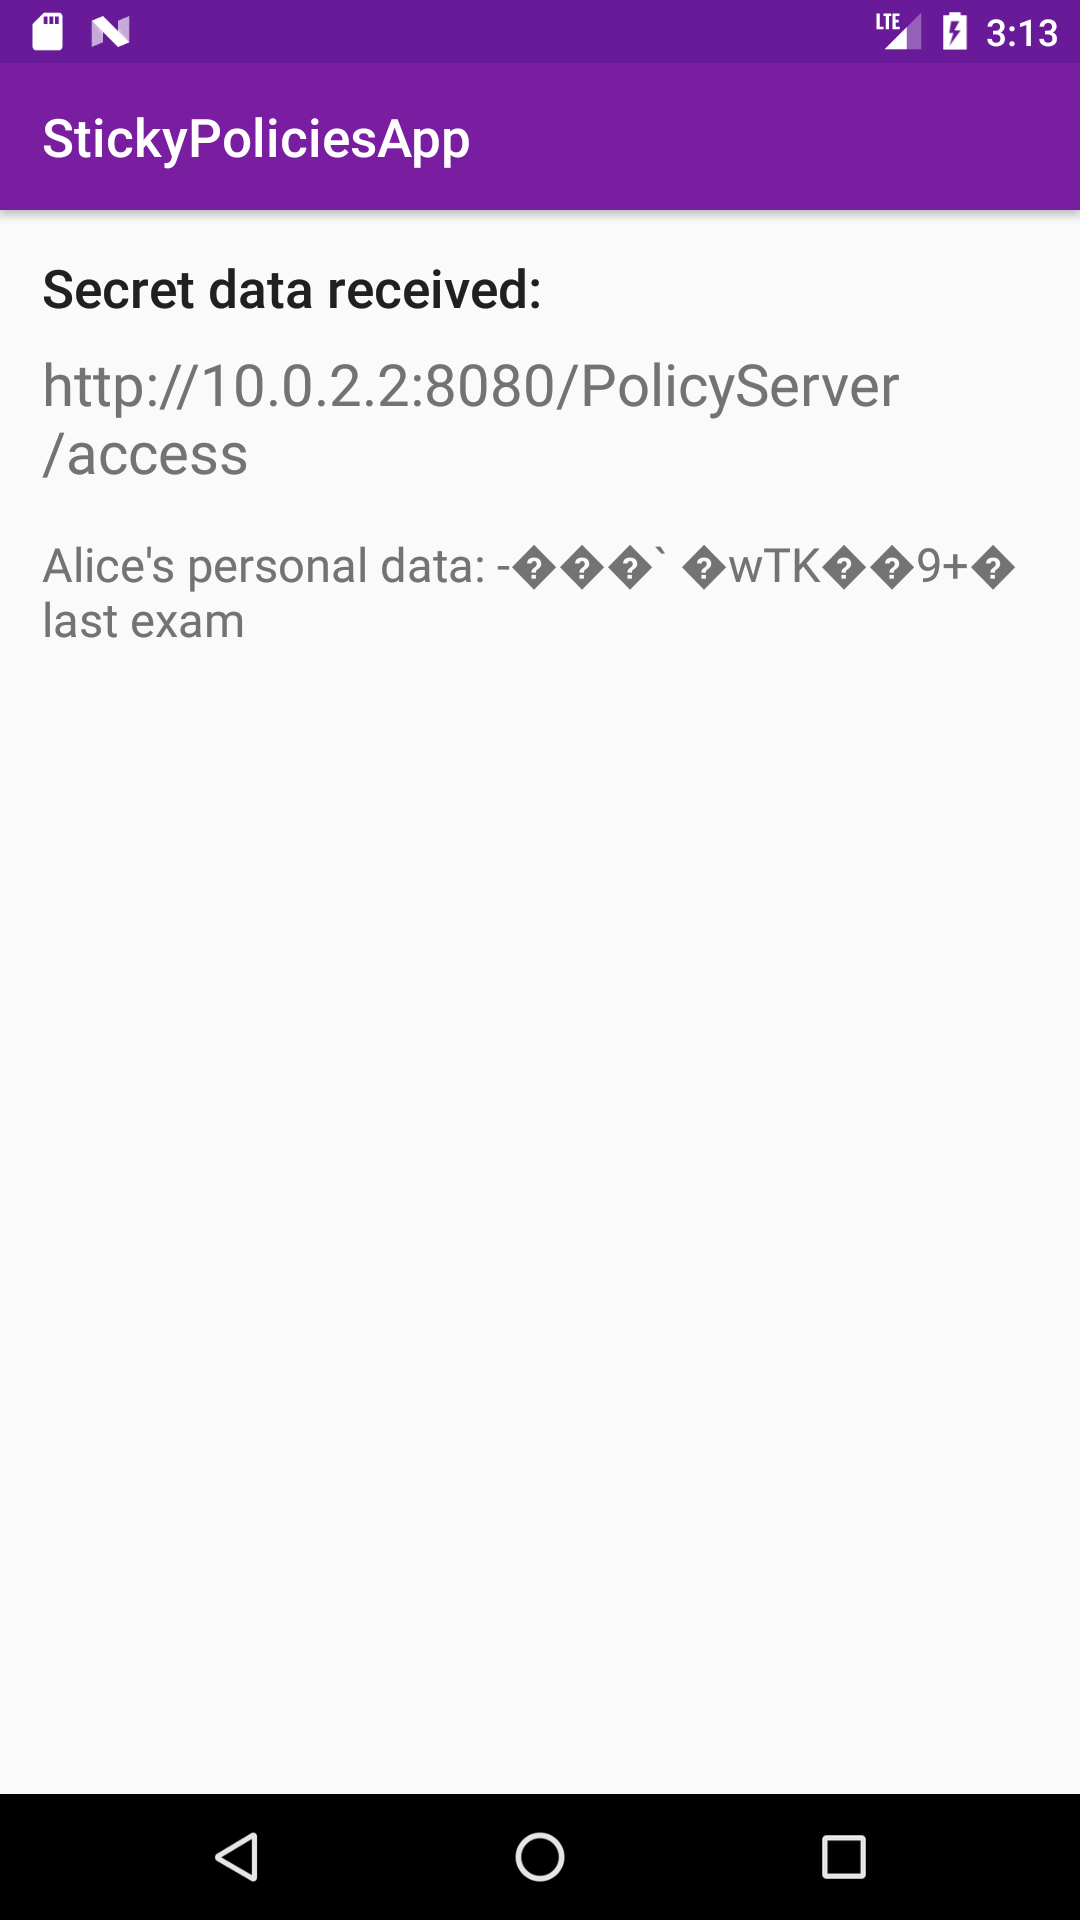
\includegraphics[width=0.35\linewidth]{DecryptCBCInvalidIV.png}
	\caption{Decrypted text in Bob's device.}
	\label{fig:DecryptCBCInvalidIV}
\end{figure}

The AES/CBC encryption scheme does not include integrity protection, meaning that a potential attacker could manipulate the encrypted data without Bob knowing it. The attacker would though have to forge a specific encrypted text, because \texttt{cipher.doFinal()} will otherwise throw exceptions as \texttt{BadPaddingException} if the encrypted text is not properly padded or the provided symmetric key is incorrect (for the provided text). Differently, if the attacker manages to substitute the key sent from the Trusted Authority with a forged key, and also manipulates the encrypted data received by Bob with a correspondingly forged text, the encryption succeeds. This situation should never happen under the assumption that the connection is secure.

Data integrity could be realized with a MAC scheme: encrypted data could be signed by Alice before sharing, yet presenting issues on both security and efficiency of the operation. A better solution could be signing the message digest, which has a fixed size and would not introduce security weaknesses nor inefficiency in computation and bandwith consumption.

In cases in which the required level of security is higher and integrity is necessary in addition to confidentiality, another solution may involve the AES/GCM/NOPADDING encryption offered by the Bouncy Castle provider. GCM stands for Galois/Counter Mode, which is a mode of operation for symmetric block ciphers providing authenticated encryption (Authenticated Encryption with Associated Data, AEAD, as described in \cite{rfc5116}). From the specification we understand that it is possible to use AES/GCM with keys either 128 or 256 bits long, and that the operations of authenticated encryption and decryption both need a secret key, a nonce, a plain or obscured text and the associated data.

From the code shown in Appendix \ref{appendixC} we can see that GCM encryption mode can be only implemented on devices which support API level 19 or higher, while AES/CBC has no limitation in this sense. Moreover, GCM would require a protocol redefinition to share the associated data: they account for authenticity and they are necessary, together with the nonce, in the decryption process.

\section{Security Considerations in Android}
When designing the security of an Android application, the first stage involves writing a correct Manifest. It is important not to give any unnecessary permission to the app, and eventually ask for runtime permissions if the API level allows it.

In this project, the only required permission is

\lstinline[language=XML]!<uses-permission android:name="android.permission.INTERNET" />!

\noindent to establish communications with the Trusted Authority web server and with other peers and services. As it is, no other permission is required, but were the app to be further developed, additional permissions may be necessary, as for example \texttt{READ\_EXTERNAL\_STORAGE}.

Another important security consideration concerns networking: in this project work, the web server is hosted at localhost thanks to the Apache Tomcat container, but in a real-world use case the implementation will differ, thus requiring a few changes also in the Android application. These edits involve secure networking: using \texttt{HttpsURLConnection} instead of \texttt{HttpURLConnection} together with \texttt{SSLSocket} to implement encrypted socket-level communication. This would make concrete our initial hypothesis of a secure communication channel.

In case this project is used with an actual Certification Authority, it will be necessary to define a Network Security Configuration for the considered CA, and to properly store keys in the Android \texttt{KeyStore}.
	\chapter{Performance and Conclusions}
\label{chapter4}
\thispagestyle{empty}

\noindent We have presented a project work on Information Security in which we tackle the matter of privacy and personal data sharing on mobile devices. In this context, we provide a tool control how data is shared in terms of recipients and scope of use: by implementing \textit{Sticky Policies} it is possible to describe detailed and fine-grained constraints for each shared file. \textit{Sticky Policies} are metadata that sticks to the data they describe through the application of cryptographic processes, and provided that third parties are trusted and will not illicitly share personal data with others, \textit{Sticky Policies} will always travel together with the data they refer to.

To obtain data access, third parties must ask a Trusted Authority and may be subject to its examination, aimed at assessing the service's reliability.

In this work, we have implemented both a data owner and a data consumer, who communicate through an Android device application; the Trusted Authority is represented by a web server in Java, which exposes the aforementioned functionalities on Java servlets.

Let us now observe the performance of the StickyPoliciesApp using the Android Profiler available within Android Studio. The Android Profiler shows CPU, memory and network usage with the passing of time, but can be used only if the Android OS is 5.0 or higher (Lollipop): thus, it is not possible to test the application on a concrete device and we will just show results regarding the Android emulator.

Our first experiment is very simple: we suppose Alice wants to share a very short string of data. We test the application using as input \texttt{I cheated during last exam} (which counts 5 words and 26 characters), a string so simple that it could be the data owner Social Security Number, credit card number and pin, or Netflix username and password. As we can see from Figure \ref{fig:performance-5words}, we have two network usage peaks both in download and upload (avg speed 5KB/s) which match certificate sharing between client and server, followed by a higher peak corresponding to Alice sharing her encrypted data to Bob (avg speed 20KB/s UL, 3KB/s DL) and him asking the Trusted Authority to be granted access.

\begin{figure}
	\centering
	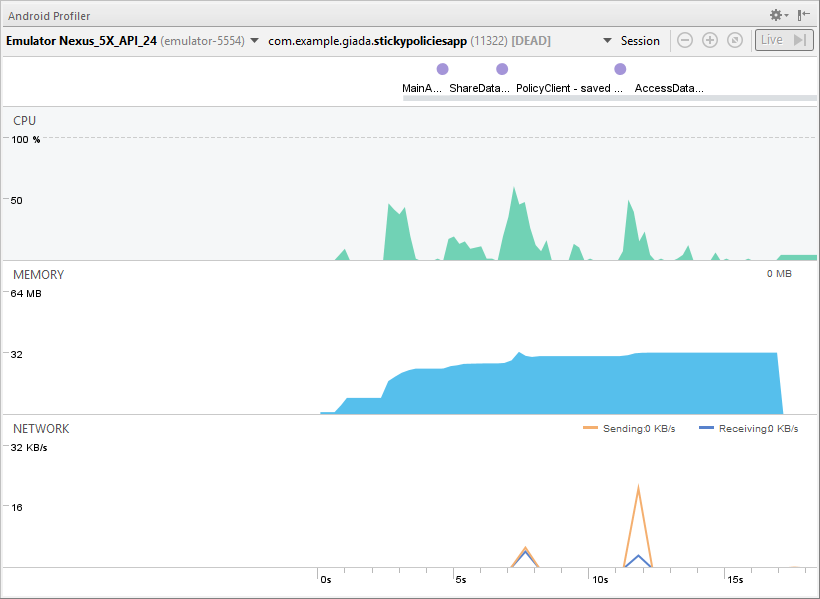
\includegraphics[width=0.95\linewidth]{Performance-5words.png}
	\caption{StickyPoliciesApp test with 5 words processing.}
	\label{fig:performance-5words}
\end{figure}

For what concerns CPU usage, we have three main peaks of duration lower than a second and occupation between 30\% and 50\%. The memory is mainly allocated for code and java usage, and it goes from 9MB at the instantiation of \texttt{MainActivity} to 32MB when \texttt{AccessDataActivity} terminates.

Next, we slightly increase the difficulty of the experiment, sharing a text document of 101 words and 605 characters. Network usage is equally divided in two moments of comparable magnitude: approximately 5KB/s in DL and UL followed by 17KB/s in UL and 2KB/s in DL. Memory usage has increased of about 10MB from the previous experiment, similarly divided between Java and code memory usage. CPU bursts have increased in number, but the percentage is usually around 25\% and the timespan of each burst is approximately 10 ms long; three main bursts are still present. Graphs from the Android Profiler are shown in Figure \ref{fig:performance-100words}.

Finally, we share a text with 1000 words (for a total count of 6804 characters): as we can observe from Figure \ref{fig:performance-1000words}, network usage radically increase, transmitting up to 91.8KB/s UL, 4KB/s DL when sharing data between Alice and Bob - this communication takes about 20 ms.Memory usage increases linearly, starting from 20MB at the instantiation to 37MB when the last activity stops. We can observe also more frequent CPU bursts: on average, the intensity has little increase in percentage, but the highest peaks reach up to 60\% even though they last less than a second.

A different approach

	\clearpage{\pagestyle{empty}\cleardoublepage}
	\addcontentsline{toc}{chapter}{Bibliography}
	\bibliographystyle{plainurl}
	\bibliography{bibl_tesi}
	
	\appendix
	
	\pagestyle{fancy} 
	\fancyfoot{}                                               
	\renewcommand{\chaptermark}[1]{\markboth{\appendixname\ \thechapter.\ #1}{}} 
	\renewcommand{\sectionmark}[1]{\markright{\thesection.\ #1}}         
	\fancyhead[LE,RO]{\bfseries\thepage}    
	
	\fancyhead[RE]{\bfseries\leftmark}    
	\fancyhead[LO]{\bfseries\rightmark}     
	\renewcommand{\headrulewidth}{0.3pt} 
	
	\chapter{XSD Grammar for Sticky Policies}
\label{appendiceA}
\thispagestyle{empty}

\lstinputlisting[language=XML]{PKIstickypolicy.xsd}

	\chapter{Java Pairing Based Cryptography Library}
\label{appendixB}
\thispagestyle{empty}

\noindent Here are reported the complete classes from \cite{ISCC:DecIov11}, mentioned in chapter \ref{chapter3}.

In this class we have a \texttt{main} function to show a sample usage of IBE cryptography.
\lstinputlisting[caption={AHIBEDIP10.class},language=java]{AHIBEDIP10-complete.java}
	
This class shows which methods are called when encrypting and decrypting.
\lstinputlisting[caption={PairingKeyEncapsulationMechanism.class},language=java]{PairingKeyEncapsulationMechanism-complete.java}

\lstinputlisting[caption={Excerpt from PairingAsymmetricBlockCipher class},label={PairingAsymmetricBlockCipher},language=java]{PairingAsymmetricBlockCipher-complete.java}
	\chapter{GCM Encryption Example}
\label{appendixC}
\thispagestyle{empty}

\lstinputlisting[language=java]{GCMEncryption.java}
	\chapter{Android Profiler Graphs}
\label{appendixD}
\thispagestyle{empty}
\noindent Full phone specifications provided by AVD Manager:
\texttt{Name: Nexus\_5X\_API\_24; CPU\textbackslash ABI: Google APIs Intel Atom (x86\_64); Path: C:\textbackslash Users\textbackslash Giada\textbackslash .android\textbackslash avd\textbackslash Nexus\_5X\_API\_24.avd; Target: google\_apis [Google APIs] (API level 24); Skin: nexus\_5x; SD Card: 100M; hw.dPad: no; hw.lcd.height: 1920; runtime.network.speed: full; hw.accelerometer: yes; hw.device.name: Nexus 5X; vm.heapSize: 256; skin.dynamic: yes; 	hw.device.manufacturer: Google; hw.lcd.width: 1080; hw.gps: yes; 	hw.initialOrientation: Portrait; image.androidVersion.api: 24; hw.audioInput: yes; image.sysdir.1: system-images\textbackslash android-24\textbackslash google\_apis\textbackslash x86\_64; 	tag.id: google\_apis; showDeviceFrame: yes; hw.camera.back: emulated; hw.mainKeys: no; AvdId: Nexus\_5X\_API\_24; hw.camera.front: emulated; hw.lcd.density: 420; avd.ini.displayname: Nexus 5X API 24; hw.gpu.mode: auto; hw.device.hash2: MD5:bc5032b2a871da511332401af3ac6bb0; hw.ramSize: 1536; hw.trackBall: no; hw.battery: yes; hw.cpu.ncore: 2; hw.sdCard: yes; tag.display: Google APIs; runtime.network.latency: none; hw.keyboard: yes; hw.sensors.proximity: yes; disk.dataPartition.size: 800M; 	hw.sensors.orientation: yes; avd.ini.encoding: UTF-8; hw.gpu.enabled: yes }

\begin{figure} [hb]
	\centering
	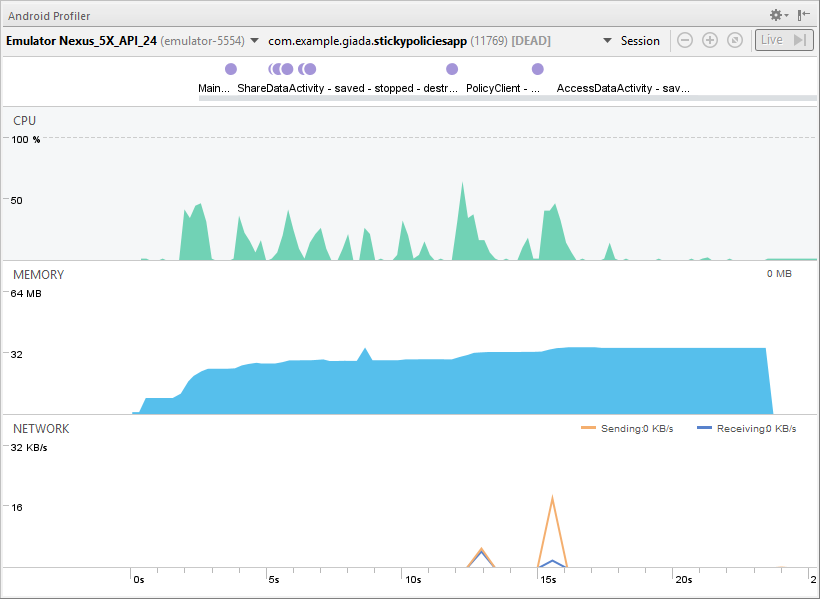
\includegraphics[width=0.55\linewidth]{Performance-100words.png}
	\caption{StickyPoliciesApp test with 101 words processing.}
	\label{fig:performance-100words}
\end{figure}
\begin{figure}
	\centering
	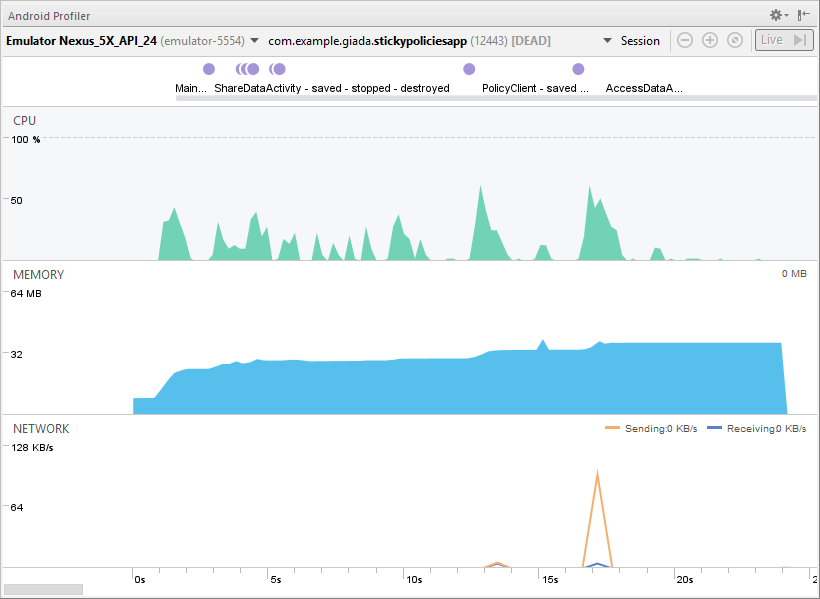
\includegraphics[width=0.55\linewidth]{Performance-1000words.png}
	\caption{StickyPoliciesApp test with 1000 words processing.}
	\label{fig:performance-1000words}
\end{figure}
\begin{figure}
	\centering
	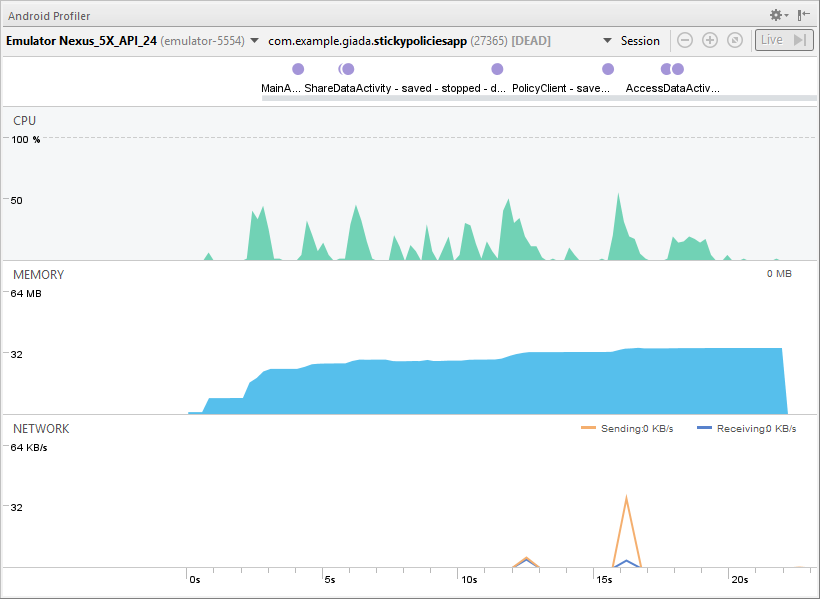
\includegraphics[width=0.55\linewidth]{Performance-100words-policy.png}
	\caption{StickyPoliciesApp test with 101 words processing and a more complex policy.}
	\label{fig:performance-100words-policy}
\end{figure}
\begin{figure}
	\centering
	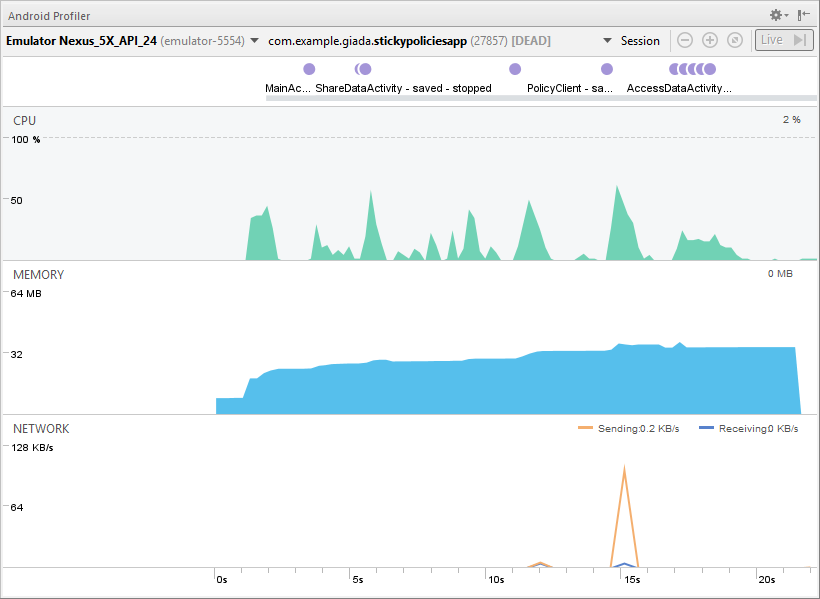
\includegraphics[width=0.55\linewidth]{Performance-1000words-policy.png}
	\caption{StickyPoliciesApp test with 1000 words processing and a more complex policy.}
	\label{fig:performance-1000words-policy}
\end{figure}
\begin{figure}
	\centering
	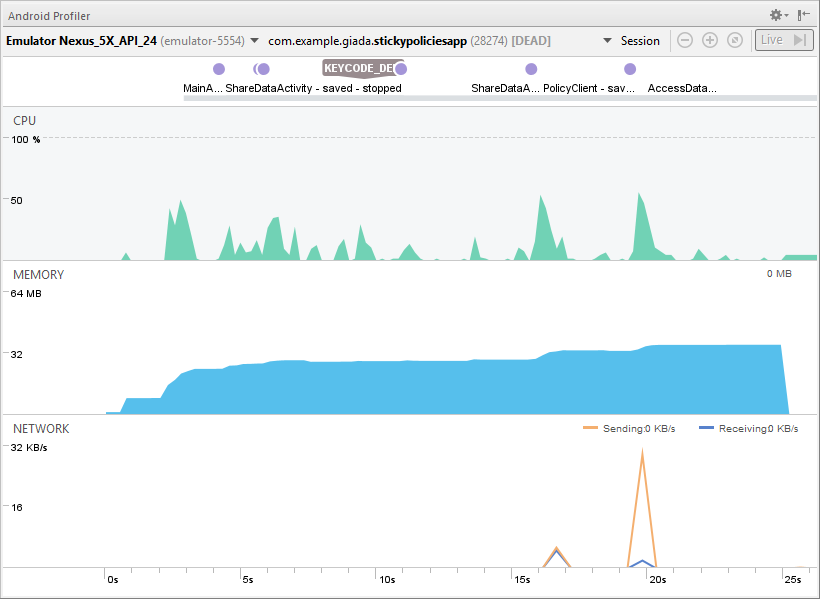
\includegraphics[width=0.55\linewidth]{Performance-image.png}
	\caption{StickyPoliciesApp test with image processing.}
	\label{fig:performance-image}
\end{figure}
\begin{figure}
	\centering
	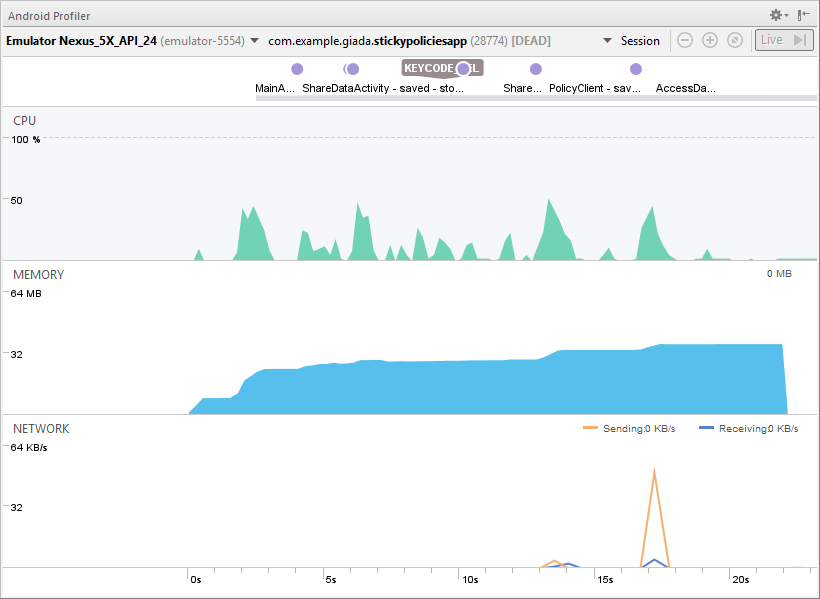
\includegraphics[width=0.55\linewidth]{Performance-image-policy.png}
	\caption{StickyPoliciesApp test with image processing and a more complex policy.}
	\label{fig:performance-image-policy}
\end{figure}

\end{document}
